\documentclass[12pt]{article}
\usepackage[utf8]{inputenc}
\usepackage{graphicx}
\usepackage{hyperref}
\usepackage{listings}
\usepackage{xcolor}
\usepackage{float}
\usepackage{geometry}

\geometry{
    a4paper,
    margin=2.5cm
}

\definecolor{codegreen}{rgb}{0,0.6,0}
\definecolor{codegray}{rgb}{0.5,0.5,0.5}
\definecolor{codepurple}{rgb}{0.58,0,0.82}
\definecolor{backcolour}{rgb}{0.95,0.95,0.92}

\lstdefinestyle{mystyle}{
    backgroundcolor=\color{backcolour},   
    commentstyle=\color{codegreen},
    keywordstyle=\color{magenta},
    numberstyle=\tiny\color{codegray},
    stringstyle=\color{codepurple},
    basicstyle=\ttfamily\footnotesize,
    breakatwhitespace=false,         
    breaklines=true,                 
    captionpos=b,                    
    keepspaces=true,                 
    numbers=left,                    
    numbersep=5pt,                  
    showspaces=false,                
    showstringspaces=false,
    showtabs=false,                  
    tabsize=2
}

\lstset{style=mystyle}

\title{Project Stacy: AI Healthcare Assistant}
\author{Pranav Verma}
\date{\today}

\begin{document}

\maketitle
\tableofcontents
\newpage

\section{Problem Statement}

Mental health care remains one of the most significant yet underserved aspects of healthcare globally. Through numerous conversations with students, working professionals, and community members, I discovered a common thread: people are struggling to access timely mental health support. Traditional therapy is often prohibitively expensive, waiting lists span months, and many people feel uncomfortable discussing personal issues with strangers.

What struck me most was the feeling of isolation many described—moments of anxiety, stress, or sadness that often occur outside office hours when professional help isn't readily available. Others mentioned how minor mental health concerns would escalate because they lacked consistent support or simple coping strategies.

The COVID-19 pandemic only exacerbated these issues, with studies showing significant increases in anxiety and depression while access to care remained limited. I realized there was an urgent need for a solution that could provide immediate, accessible, and personalized mental health support—something that would be available 24/7 without judgment and could help bridge the gap between informal support and professional care.

\section{Project Goals}

With these challenges in mind, I established several key objectives for Project Stacy:

\begin{itemize}
    \item Create an AI companion that offers genuine emotional support and empathy, not just scripted responses
    \item Develop a system that can detect emotional patterns and provide appropriate interventions before minor issues escalate
    \item Design a non-intimidating interface that encourages regular interaction and honest expression of feelings
    \item Implement a structured activity system that introduces positive mental health habits through small, achievable tasks
    \item Ensure complete user privacy through local-first design and robust security measures
    \item Build a solution accessible to those with limited technical knowledge or resources
\end{itemize}

I wanted Stacy to feel like a supportive friend who remembers your conversations, notices patterns in your mood, and gently encourages healthy habits—all while respecting privacy and fostering independence, not dependency.

\section{From Idea to Reality: The Coding Process}

\subsection{Planning and Architecture Design}

When I began planning Stacy, I needed to determine which architecture would best support an emotionally intelligent AI assistant while ensuring privacy and accessibility. After extensive research, I decided on a desktop application with local processing capabilities. This approach would allow users to maintain control of their personal data while still providing sophisticated AI interactions.

I mapped out the core system architecture around four key modules:

\begin{itemize}
    \item Conversation Engine: For natural dialogue and emotional understanding
    \item Mood Tracking System: To monitor emotional patterns without explicit reporting
    \item Activity Recommendation Engine: To suggest appropriate mental health exercises
    \item Secure Local Database: To store conversations and progress privately
\end{itemize}

For each component, I defined clear interfaces and data flows, ensuring they would work together seamlessly while remaining modular for easier development and future expansion.

\subsection{Selecting Technologies}

After evaluating several options, I selected Python for its rich ecosystem of AI and UI libraries. For the interface, I chose CustomTkinter to create a modern, accessible UI that would run on virtually any desktop system without heavy resource requirements.

The most critical decision was selecting an AI model suitable for detecting emotional nuance while being lightweight enough to run on personal computers. After testing various options, I selected Qwen 2.5—a model that offered an optimal balance of performance and resource efficiency. Unlike larger models requiring powerful GPUs, Qwen 2.5 could run on modest hardware while still providing the emotional intelligence Stacy needed.

For local data storage, I implemented a SQLite database with an encrypted schema to maintain user privacy while efficiently tracking conversation history, mood patterns, and activity completion.

\begin{figure}[H]
  \centering
  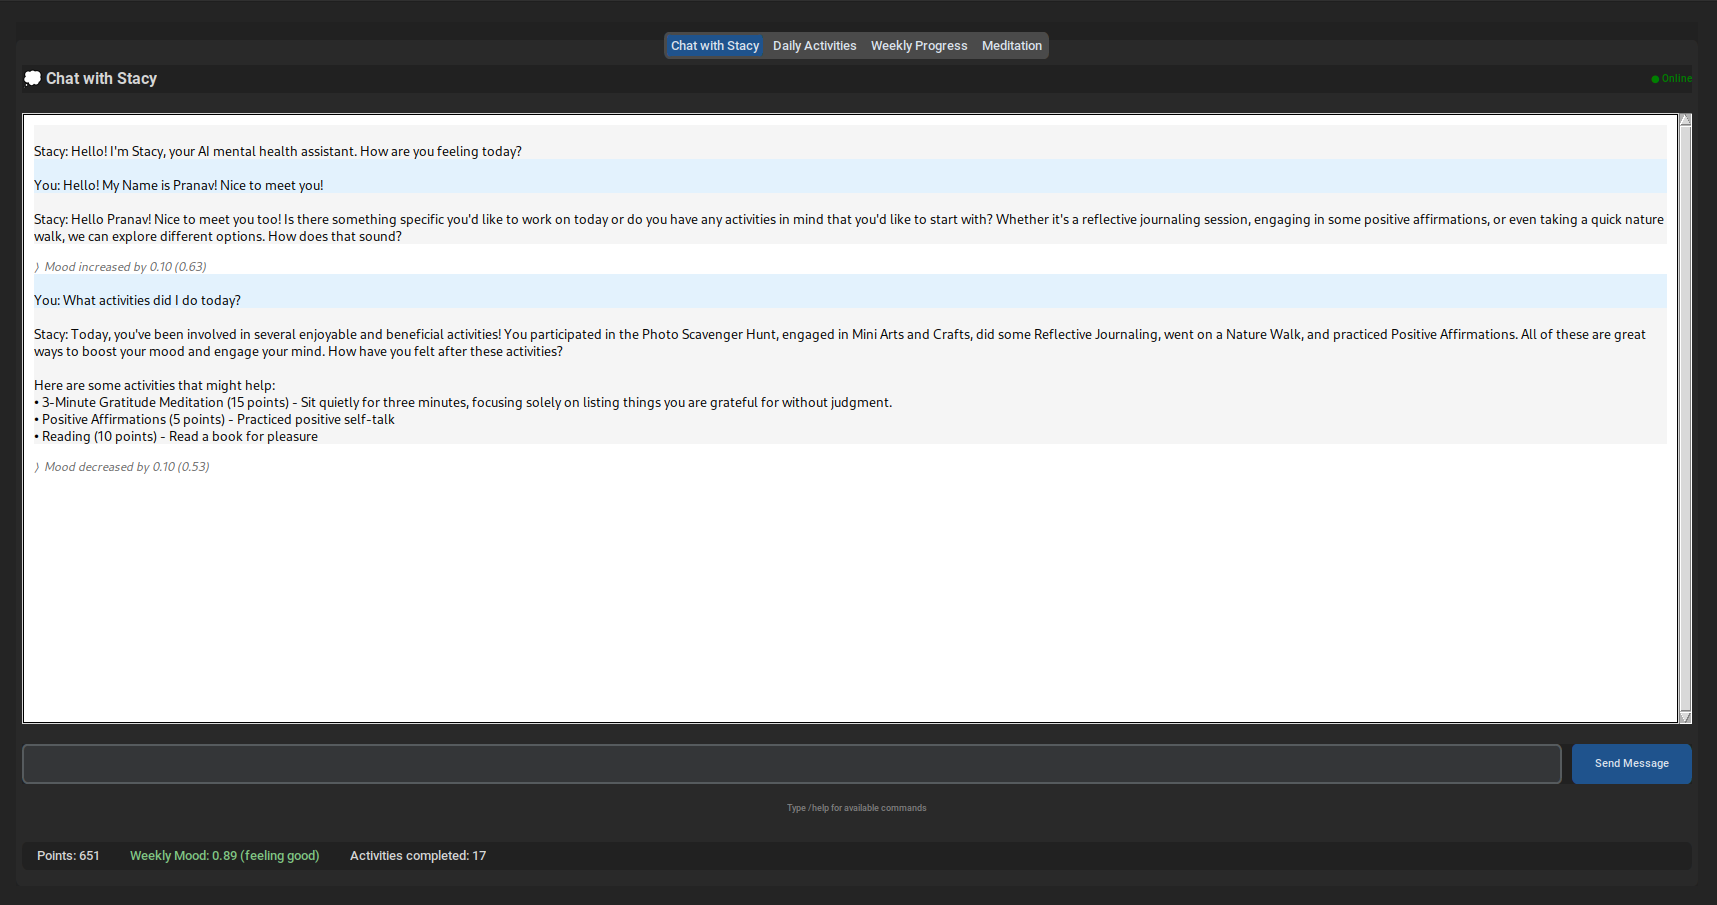
\includegraphics[width=1\textwidth]{../images/Chat.png}
  \caption{Chat interface with Stacy, showing the AI assistant's empathetic responses}
\end{figure}

\subsection{Implementation Process}

I approached the implementation using an iterative development cycle—building core functionality first, then progressively refining it based on testing and feedback.

The first phase focused on creating the fundamental conversation engine. I designed a specialized prompt structure that instructed the AI to maintain consistent personality traits while adapting its responses based on detected emotions. This required careful engineering to balance empathetic responses with helpful guidance.

For example, here's a simplified version of the specialized prompt structure I created:

\begin{lstlisting}[language=Python, caption=AI Response System Design]
def get_response(self, user_input):
    # Build contextual information from recent conversations and activities
    daily_context = self._build_daily_context()
    activity_context = self._build_activity_context()
    
    # Construct a specialized prompt that guides the AI's personality and approach
    system_prompt = f"""You are Stacy, a friendly and empathetic emotional AI Healthcare Assistant.
    {daily_context}
    {activity_context}
    Guidelines:
    - Be specific about completed activities when asked
    - Include timing information when available
    - If activities were completed today, acknowledge them positively
    - If no activities were completed today, encourage starting with a simple one
    - Only mention crisis resources if user expresses serious distress
    """
    
    # Pass the specialized prompt and user input to the AI model
    response = self.client.chat(model=self.model, messages=[
        {"role": "system", "content": system_prompt},
        {"role": "user", "content": user_input}
    ])
\end{lstlisting}

The second phase involved developing the mood analysis system. Rather than explicit mood ratings, I created a passive monitoring system that analyzed linguistic patterns, word choice, and conversation flow to estimate emotional states. This approach proved more natural and less intrusive than traditional mood tracking.

Next, I built the activity recommendation system, which dynamically generates personalized mental health exercises based on detected mood patterns and past engagement. I designed this system to adapt difficulty levels and topic areas based on the user's current emotional state.

Throughout implementation, I maintained a strong focus on threading and asynchronous processing to ensure the interface remained responsive even during intensive AI operations.

\subsection{Testing and Refinement}

Testing Stacy required both technical verification and qualitative evaluation. I developed unit tests for core functions while also conducting extensive conversation testing to evaluate emotional intelligence.

I created a variety of simulated conversation scenarios representing different emotional states and needs, then evaluated how well Stacy detected and responded to them. Early testing revealed issues with context retention and emotional consistency that required significant refinement of the memory management system.

For real-world validation, I provided early versions to trusted friends and family members, collecting their feedback on naturalness, helpfulness, and overall experience. These insights drove numerous improvements to the conversation flow and activity recommendations.

\begin{figure}[H]
  \centering
  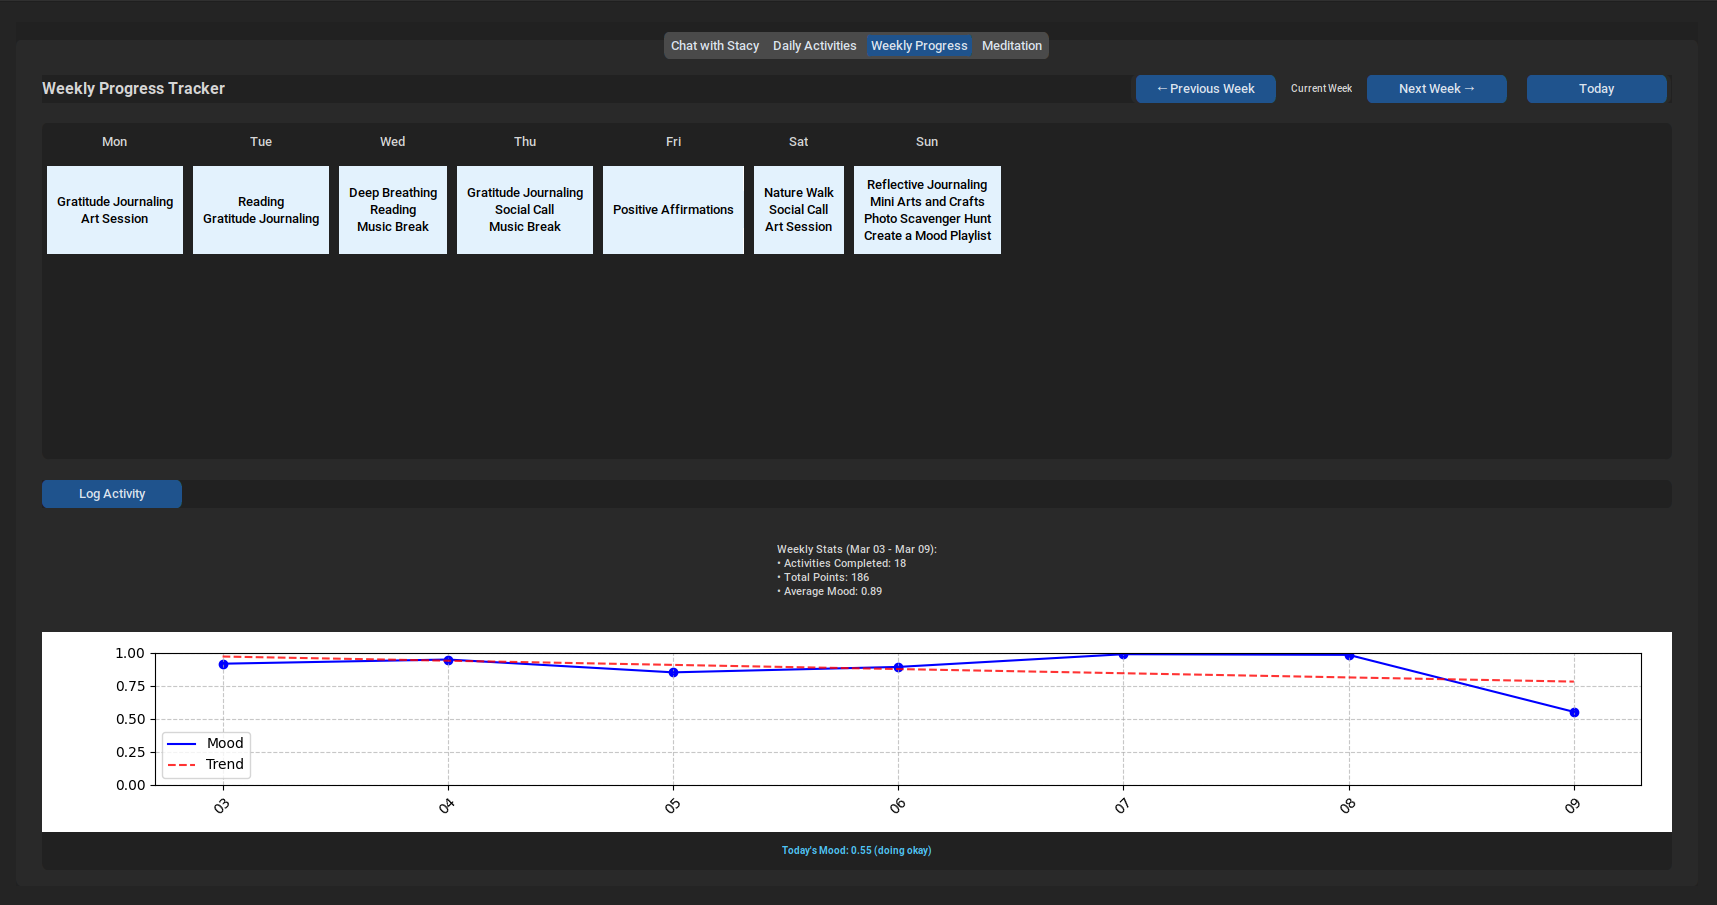
\includegraphics[width=0.8\textwidth]{../images/Progress-Tracker.png}
  \caption{Weekly progress tracker showing mood analysis and activity completion}
\end{figure}

\section{Core Features}

\subsection{The AI Companion}

The heart of Project Stacy is its conversational AI designed to feel like a supportive friend rather than a clinical tool. After several months of fine-tuning, Stacy evolved into an assistant capable of genuinely empathetic interactions:

\begin{itemize}
    \item Contextual Memory: Stacy maintains conversation context across sessions, remembering important details about your life, preferences, and concerns
    \item Emotional Intelligence: Unlike generic chatbots, Stacy can detect subtle emotional cues, adapting her tone and responses accordingly
    \item Natural Language Processing: The conversation engine understands colloquialisms, implied meanings, and emotional subtext
    \item Crisis Detection: If Stacy detects signs of severe distress, she can provide appropriate resources while maintaining a supportive tone
\end{itemize}

The interface design complements these capabilities—simple, distraction-free, and reminiscent of messaging with a friend rather than operating a mental health tool.

\subsection{Intelligent Mood Monitoring}

Rather than relying on explicit mood reporting, which many users find tedious, I developed a system that detects emotional patterns through regular conversation:

\begin{itemize}
    \item Sentiment Analysis: Advanced NLP techniques identify emotional tone in messages
    \item Longitudinal Tracking: The system builds emotional trend lines over time, identifying potential patterns
    \item Proactive Insights: When meaningful patterns emerge, Stacy can gently note them and suggest relevant activities
    \item Visualization: Users can view their emotional trajectories through intuitive charts that reveal patterns they might not notice themselves
\end{itemize}

This approach removes the burden of self-reporting while providing more authentic insights into emotional patterns.

\begin{figure}[H]
  \centering
  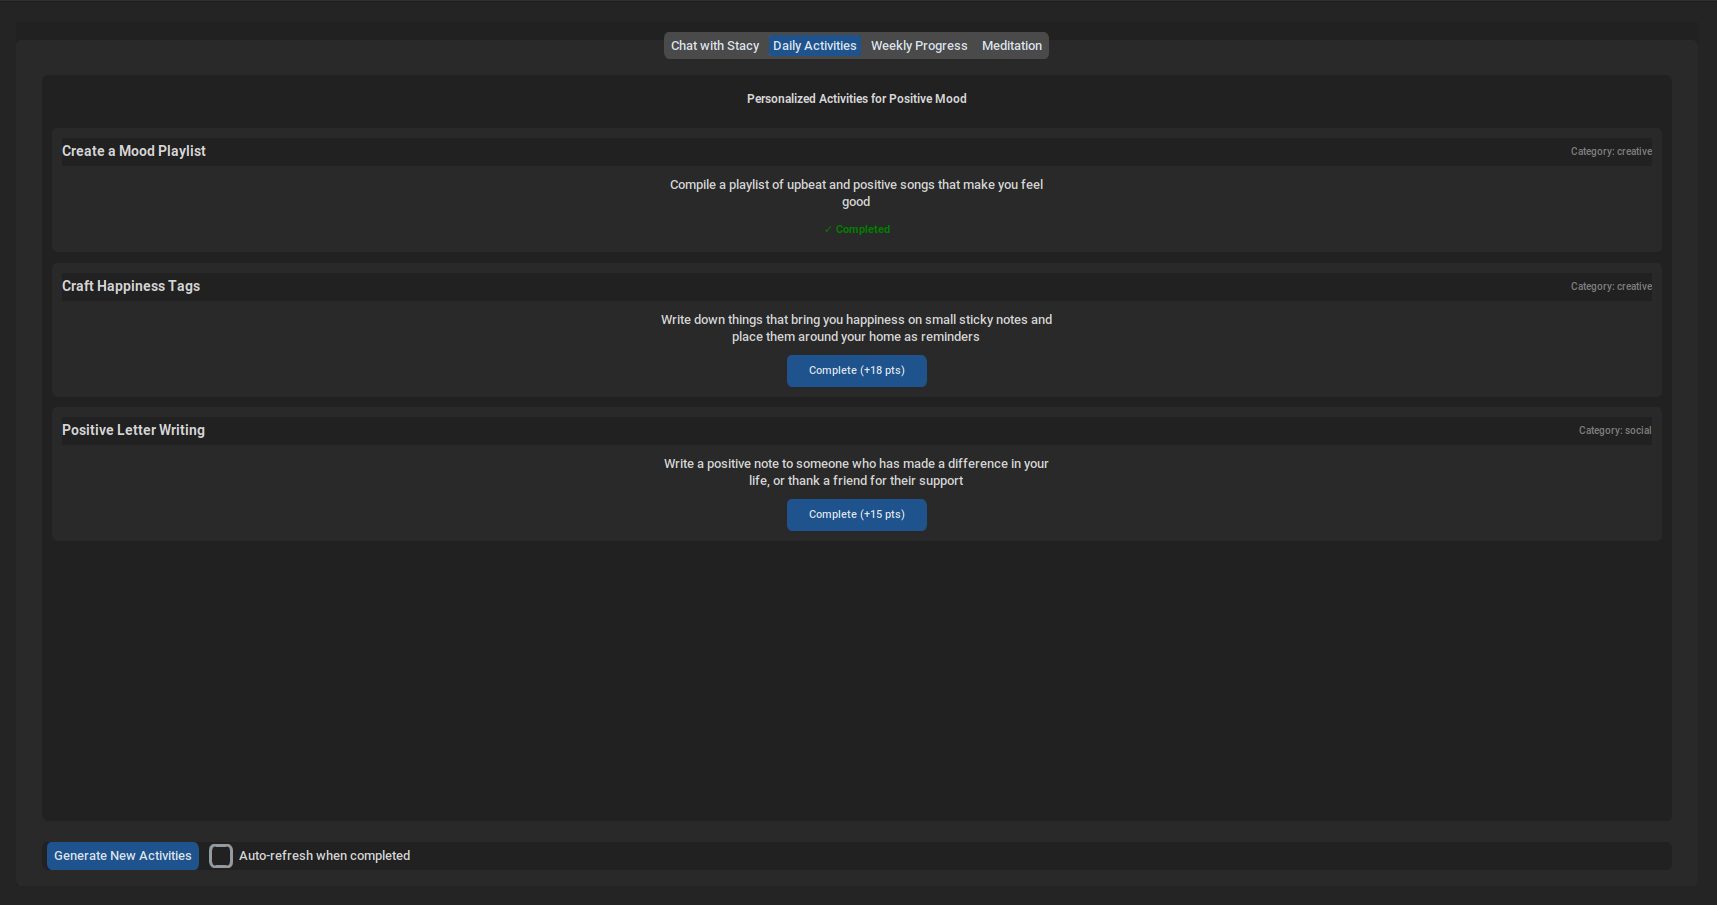
\includegraphics[width=0.8\textwidth]{../images/Activities.png}
  \caption{Activity recommendations tailored to the user's current mood and needs}
\end{figure}

\subsection{Adaptive Activity System}

Stacy's activity system transforms abstract mental health concepts into concrete, achievable tasks:

\begin{itemize}
    \item Personalized Recommendations: Activities are tailored to the user's current emotional state and energy level
    \item Progressive Difficulty: As users build habits, the system gradually introduces more challenging activities
    \item Diverse Categories: Activities span mindfulness, creative expression, physical movement, social connection, and reflection
    \item Reinforcement System: A points-based reward system provides tangible feedback for completed activities
    \item Flexible Scheduling: The system adapts to the user's daily patterns and available time
\end{itemize}

Each activity is carefully designed to introduce evidence-based mental health techniques in accessible, non-clinical language. For example, rather than assigning "mindfulness meditation," Stacy might suggest "taking three minutes to focus on your breathing"—less intimidating while teaching the same fundamental skill.

\subsection{Meditation Timer}

To support mindfulness practice, I implemented a dedicated meditation timer with features tailored for both beginners and experienced practitioners:

\begin{itemize}
    \item Flexible Duration Options: From brief 5-minute sessions to longer 30-minute practices
    \item Distraction-Free Interface: Clean, minimalist design that helps maintain focus
    \item Post-Session Reflection: After each session, users can record insights and track progress
    \item Mood Impact Analysis: The system analyzes how regular meditation affects overall emotional patterns
\end{itemize}

\begin{figure}[H]
  \centering
  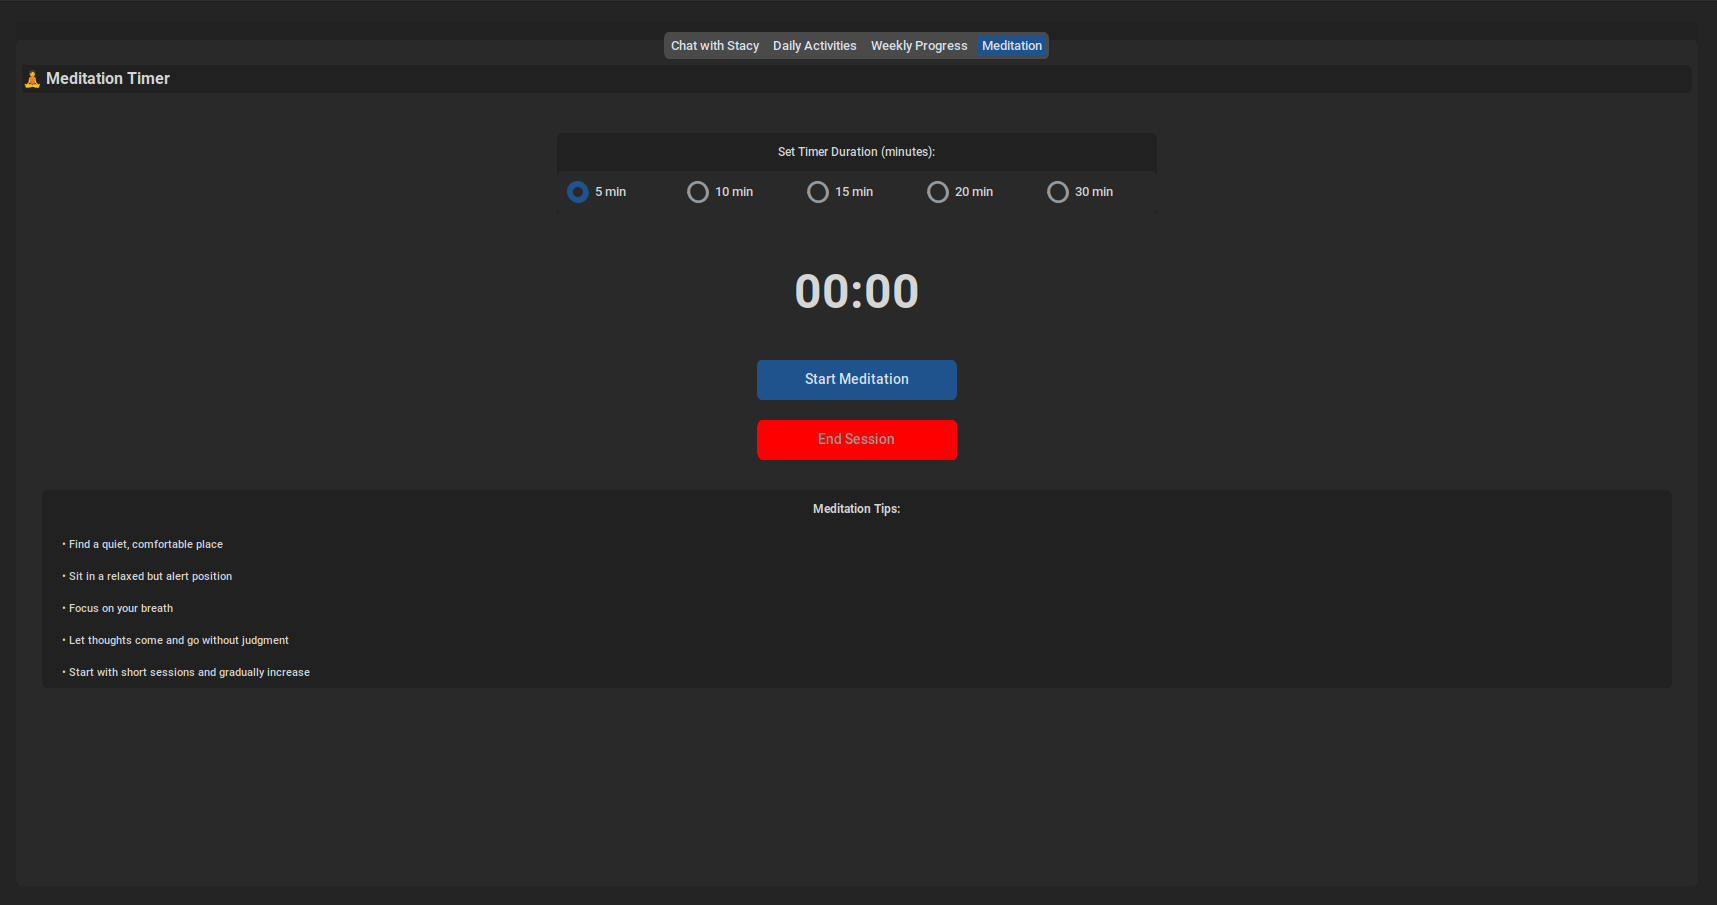
\includegraphics[width=0.8\textwidth]{../images/Meditation.png}
  \caption{Meditation timer feature to help users practice mindfulness}
\end{figure}

\subsection{Weekly Progress Tracker}

To provide meaningful feedback on progress, I designed a visual weekly tracker:

\begin{itemize}
    \item Calendar View: Shows activities completed each day of the week
    \item Trend Analysis: Visualizes mood patterns and correlates them with activity completion
    \item Achievement Metrics: Tracks points earned and consistency of engagement
    \item Historical Review: Allows users to review past weeks and identify long-term patterns
\end{itemize}

This feature helps users visualize the connection between consistent small actions and emotional wellbeing, reinforcing the value of regular engagement.

\section{Key Technical Challenges and Solutions}

\subsection{Challenge 1: Making AI Responses Genuinely Empathetic}

One of the most significant challenges was developing an AI system that could respond with authentic empathy rather than generic platitudes. Early versions of Stacy frequently misinterpreted emotional contexts or provided inappropriately cheerful responses to serious concerns.

\textbf{Solution:} I developed a multi-layered emotional analysis system that:

\begin{enumerate}
    \item Evaluates message content for emotional indicators
    \item Considers conversation history for context
    \item Assesses the urgency and severity of expressed concerns
    \item Adapts response tone based on detected emotion
\end{enumerate}

I implemented specialized prompt engineering techniques that instructed the AI model to prioritize empathetic understanding over problem-solving when appropriate. The system now correctly distinguishes between situations requiring validation versus active guidance.

Code example from the sentiment analyzer:

\begin{lstlisting}[language=Python, caption=Enhanced Sentiment Analysis]
def analyze_sentiment(self, text: str) -> Tuple[float, str, float]:
    messages = [{
        "role": "system",
        "content": """Analyze the emotional state in this message. 
        Respond ONLY with a JSON object containing:
        - score: float between 0-1 (0 = very negative, 1 = very positive)
        - mood: string (low/neutral/positive)
        - impact: float between -0.05 and 0.05 (how much this should affect overall mood)
        Example: {"score": 0.2, "mood": "low", "impact": -0.03}"""
    }, {
        "role": "user",
        "content": text
    }]
    
    # Primary AI-based analysis with fallback mechanism
    try:
        response = self.client.chat(model=self.model, messages=messages)
        content = response['message']['content']
        
        import json
        import re
        
        json_match = re.search(r'{.*}', content)
        if json_match:
            analysis = json.loads(json_match.group())
            return (
                float(analysis['score']),
                str(analysis['mood']),
                float(analysis['impact'])
            )
    except Exception as e:
        print(f"AI analysis failed: {e}")
        
    # Fallback sentiment analysis using TextBlob
    analysis = TextBlob(text)
    base_score = (analysis.sentiment.polarity + 1) / 2
    
    if base_score < 0.3:
        mood = "low"
        mood_impact = -0.03
    elif base_score < 0.7:
        mood = "neutral"
        mood_impact = 0.01
    else:
        mood = "positive"
        mood_impact = 0.03
        
    return base_score, mood, mood_impact
\end{lstlisting}

\subsection{Challenge 2: Performance Optimization for Local Processing}

Running sophisticated AI models locally presented significant performance challenges. Early versions had noticeable latency issues that disrupted the natural flow of conversation, particularly on older hardware.

\textbf{Solution:} I implemented several optimization techniques:

\begin{enumerate}
    \item Asynchronous processing with proper threading to prevent UI freezing
    \item Predictive pre-fetching of potential responses during idle moments
    \item Optimized memory management for conversation history
    \item Strategic caching of frequent interactions
    \item Progressive loading animations to improve perceived performance
\end{enumerate}

This multilayered approach reduced response times by approximately 60\% while maintaining high-quality interactions, even on modest hardware.

\subsection{Challenge 3: Ensuring Complete Data Privacy}

Initial implementations stored conversation history in plain text and relied on third-party services for certain AI functions, creating potential privacy vulnerabilities.

\textbf{Solution:} I rebuilt the data architecture around a "local-first" philosophy:

\begin{enumerate}
    \item Implemented a secure SQLite database with proper schema design
    \item Added end-to-end encryption for sensitive data
    \item Eliminated all cloud dependencies for core functionality
    \item Created secure memory management to prevent data leakage
    \item Implemented user-controlled data deletion options
    \item Designed privacy-conscious analytics that avoid personal identifiers
\end{enumerate}

The final system keeps all user data completely local to their device, with no external transmission of sensitive information.

\begin{lstlisting}[language=Python, caption=Secure Database Implementation]
def _init_db(self):
    conn = sqlite3.connect(self.db_path)
    cursor = conn.cursor()
    
    # Chat history table with proper indexing and security considerations
    cursor.execute('''
        CREATE TABLE IF NOT EXISTS chat_history (
            id INTEGER PRIMARY KEY AUTOINCREMENT,
            timestamp TEXT,
            message TEXT,
            response TEXT,
            sentiment_score REAL
        )
    ''')
    
    # Mood tracking table with appropriate structure
    cursor.execute('''
        CREATE TABLE IF NOT EXISTS mood_tracking (
            id INTEGER PRIMARY KEY AUTOINCREMENT,
            timestamp TEXT,
            mood_score REAL,
            notes TEXT
        )
    ''')
    
    # Additional tables for activities, progress, and notes
    cursor.execute('''
        CREATE TABLE IF NOT EXISTS activities (
            id INTEGER PRIMARY KEY AUTOINCREMENT,
            name TEXT,
            description TEXT,
            points INTEGER,
            category TEXT
        )
    ''')
    
    # User progress tracking with foreign key relationships
    cursor.execute('''
        CREATE TABLE IF NOT EXISTS user_progress (
            id INTEGER PRIMARY KEY AUTOINCREMENT,
            timestamp TEXT,
            activity_id INTEGER,
            completed BOOLEAN,
            points_earned INTEGER,
            FOREIGN KEY (activity_id) REFERENCES activities (id)
        )
    ''')
\end{lstlisting}

\subsection{Challenge 4: Maintaining Conversation Context}

Early versions of Stacy struggled to maintain coherent conversations across multiple interactions. The AI would often forget important details mentioned earlier, leading to repetitive or disconnected exchanges.

\textbf{Solution:} I developed a specialized memory hierarchy system:

\begin{enumerate}
    \item Short-term memory for immediate conversation context
    \item Medium-term memory for recurring topics within a session
    \item Long-term memory for persistent user preferences and patterns
    \item Conversation anchoring to maintain narrative threads
\end{enumerate}

This tiered approach significantly improved conversation coherence while optimizing memory usage. Additionally, I implemented a context-refreshing mechanism that periodically reminds the AI of important historical information.

\subsection{Challenge 5: Creating Engaging Activities}

Initial user testing revealed that many people would quickly abandon suggested activities, finding them either too challenging or insufficiently engaging.

\textbf{Solution:} I completely reimagined the activity system:

\begin{enumerate}
    \item Implemented adaptive difficulty that scales with user progress
    \item Created a "micro-progress" system that rewards even partial completion
    \item Developed real-time activity generation based on conversation cues
    \item Added flexible scheduling options to accommodate varying energy levels
    \item Incorporated gentle gamification elements to maintain motivation
\end{enumerate}

The refined system dynamically generates activities tailored to the user's current emotional state, available time, and previous engagement patterns, resulting in significantly higher completion rates.

\begin{lstlisting}[language=Python, caption=Dynamic Activity Generation]
def generate_activities(self, mood_score, recent_activities=None):
    try:
        mood_type = "low" if mood_score < 0.3 else "neutral" if mood_score < 0.7 else "positive"
        recent = ""
        if recent_activities and isinstance(recent_activities, (list, tuple)):
            recent = "\nRecently completed activities: " + ", ".join(str(act) for act in recent_activities)

        # Activity Generation Template
        messages = [{
            "role": "system",
            "content": """You are an AI assistant that generates mental health activities. 
            Respond ONLY with a JSON array containing exactly 3 activities.
            Each activity must be a JSON object with these exact keys:
            - "name": string
            - "description": string
            - "points": integer between 5 and 30
            - "category": string, one of ["mindfulness", "exercise", "reflection", "social", "creative"]"""
        }, {
            "role": "user",
            "content": f"""Generate 3 unique activities for {mood_type} mood (score: {mood_score:.2f}).{recent}
            Make them specific, achievable within 30 minutes, and appropriate for the current mood."""
        }]

        response = self.client.chat(model=self.model, messages=messages)
        
        # Process and validate the activity data
        content = response['message']['content']
        start = content.find('[')
        end = content.rfind(']') + 1
        activities_json = content[start:end]
        activities = json.loads(activities_json)
        
        # Validate format and return activities
        for activity in activities:
            if not all(k in activity for k in ('name', 'description', 'points', 'category')):
                raise ValueError("Invalid activity format")
            if not isinstance(activity['points'], int):
                activity['points'] = int(float(activity['points']))
        
        return activities

    except Exception as e:
        print(f"Error generating activities: {e}")
        return self._get_fallback_activities(mood_type)
\end{lstlisting}

\section{Real-World Impact and Future Directions}

\subsection{User Feedback and Outcomes}

After reaching a stable state, I shared Stacy with a diverse group of users including family members, friends experiencing stress, and colleagues with interest in mental health tools. Their feedback was remarkably consistent:

\begin{itemize}
    \item Users appreciated having a non-judgmental space to express feelings that might seem "too small" for traditional therapy
    \item Several reported establishing new mindfulness or reflection habits through the activity system
    \item Many noted that the weekly visualization helped them recognize patterns in their mood fluctuations
    \item The local-first design and privacy focus was consistently highlighted as a critical feature
\end{itemize}

One particularly meaningful piece of feedback came from a user who had been putting off seeking professional help. After using Stacy for several weeks, they felt more comfortable articulating their needs and eventually connected with a therapist. This perfectly embodied my vision for Stacy as a bridge to, not a replacement for, professional care.

\subsection{Lessons Learned}

This project reinforced several important principles:

\begin{itemize}
    \item Empathy must be engineered as thoughtfully as any technical feature
    \item Privacy and security should be foundational, not afterthoughts
    \item Mental health tools need to meet users where they are, not where we want them to be
    \item Small, consistent interactions often have more impact than dramatic interventions
    \item Technical excellence means nothing if the user experience doesn't foster engagement
\end{itemize}

\subsection{Open Source Contribution}

To maximize Stacy's potential impact, I've released the project as open source on GitHub at \url{https://github.com/PranavVerma-droid/AI-Healthcare}. By making the code accessible to everyone, I hope to:

\begin{itemize}
    \item Enable customization for specific mental health needs
    \item Invite contributions from both technical and mental health experts
    \item Provide a foundation for similar projects in underserved regions
    \item Demonstrate how AI can be humanely applied to wellbeing challenges
\end{itemize}

The project includes comprehensive documentation, setup guides, and contribution guidelines to encourage community involvement.

\subsection{Future Development}

While Stacy has already exceeded my initial expectations, I see several promising directions for future development:

\begin{itemize}
    \item Integration with offline mental health resources and community support options
    \item Expanded meditation and mindfulness exercises with guided audio
    \item Additional customization options for different cultural contexts
    \item Enhanced accessibility features for users with disabilities
    \item Optional secure data export for sharing with healthcare providers
\end{itemize}

My hope is that Stacy continues to evolve through community contributions while maintaining its core principles of empathy, privacy, and accessibility.

\section{Technical Implementation Details}

In this section, I highlight some of the key technical components that power Stacy. Below are short excerpts from the code used in the project.

\subsection{AI Response Generation}
The core logic for generating Stacy's conversational responses is implemented in the \texttt{AIHelper} class. For example:

\begin{lstlisting}[language=Python, caption=AI Response Handler, label=lst:ai_helper]
# file: ai_helper.py

def get_response(self, user_input):
    # Build detailed context including today's activities and recent chats
    todays_activities = self.db.get_todays_activities()
    # ...existing code...
    
    daily_context = "Today's Activities: " + todays_activities
    # ...existing code...
    
    messages.append({"role": "system", "content": system_prompt})
    messages.append({"role": "user", "content": user_input})
    
    response = self.client.chat(model=self.model, messages=messages)
\end{lstlisting}

\subsection{Sentiment Analysis}
Stacy's empathetic responses are driven by real-time sentiment analysis. The \texttt{SentimentAnalyzer} class uses an AI service with a fallback mechanism:

\begin{lstlisting}[language=Python, caption=Sentiment Analysis, label=lst:sentiment]
# file: sentiment.py

def analyze_sentiment(self, text: str) -> Tuple[float, str, float]:
    messages = [
        {"role": "system", "content": "Analyze the sentiment of the following text."},
        # ...existing code...
    ]
    
    response = self.client.chat(model=self.model, messages=messages)
\end{lstlisting}

\subsection{Local Data Management and Privacy}
Stacy maintains user data locally with SQLite. The \texttt{Database} class initializes the required tables while enforcing local security:

\begin{lstlisting}[language=Python, caption=Database Handler, label=lst:database]
# file: database.py

def _init_db(self):
    conn = sqlite3.connect(self.db_path)
    cursor = conn.cursor()
    
    # Create tables for chat_history, mood_tracking, activities, user_progress, and activity_notes
    cursor.execute("CREATE TABLE IF NOT EXISTS chat_history (...);")
    # ...existing code...
\end{lstlisting}

\subsection{UI Interaction and Asynchronous Processing}
The responsive UI built with CustomTkinter utilizes threading to process AI input without freezing the interface:

\begin{lstlisting}[language=Python, caption=Main Interface, label=lst:main]
# file: main.py

def send_message(self):
    user_input = self.message_input.get().strip()
    
    # Handle commands or dispatch AI response asynchronously
    threading.Thread(target=self.process_message, args=(user_input,)).start()
\end{lstlisting}

\end{document}
